\chapter{Lucr\u ari similare}

\paragraph{}
Fiind un subiect at\^ at de fierbinte care prime\c ste o mul\c time de aten\c tie din partea comunit\u a\c tii \c stiin\c tifice, existen\c ta a nenum\u arate abord\u ari \c si sisteme ligvistice inteligente este un fapt natural. \^ In prezent, exist\u a dou\u a mari abord\u ari de a genera limbaj natural. \^ In primul r\^ and, cele mai populare sunt modelele de tip reg\u asire \cite{chatbot-models}, unde r\u aspunsul este stocat \^ intr-o surs\u a de date \c si returnat pe baza unor metode de pattern matching. Cea de-a doua abordare sunt modelele generative \cite{chatbot-models}, care produc un r\u aspuns dinamic folosind diverse metode din teoria probabilit\u a\c tilor.

\section{Modele de reg\u asire}

\paragraph{}
Modelele de acest tip folosesc o surs\u a de date care con\c tine numeroase r\u aspunsuri predefinite. R\u aspunsul este ales folosind o metod\u a euristic\u a pentru o potrivire c\^ at mai bun\u a cu putin\c t\u a, lu\^ and \^ in considerare intrarea \c si contextul. Tipul de euristic\u a folosit poate fi ceva simplu precum o expresie bazat\u a pe o regul\u a de potrivire sau ceva mai complex cum ar fi un clasificator de Machine Learning \cite{retrieval-chatbots}. Se poate deduce foarte u\c sor c\u a aceste sisteme nu genereaz\u a text nou. O problem\u a uria\c s\u a a acestor modele o reprezint\u a incapacitatea de a reac\c tiona la cazuri nemai\^ intalnite pentru care nu exist\u a un r\u aspuns potrivit. Acestea au totu\c si avantajele lor. Datorit\u a sursei de date cu r\u aspunsuri create de oameni, aceste metode nu produc erori gramaticale. \^ In prezent, aceast\u a abordare este cea mai popular\u a \c si sigur\u a pentru problemele \^ in care r\u aspunsul este unul sensibil, \^ intr-un domeniu precum cel medical, de exemplu, unde r\u aspunsul trebuie s\u a provin\u a de la un specialist.

\subsection{Duolingo}

\paragraph{}
Populara aplica\c tie de \^ inv\u a\c tare a limbilor str\u aine Duolingo \cite{duolingo} (Figura 2.1) folose\c ste o abordare interesant\u a cu privire la chatbots. Aceasta dore\c ste s\u a \^ i\c si ajute utilizatorii s\u a practice o nou\u a limb\u a prin conversa\c tii cu chatbots. Av\^ and \^ in vedere c\u a o conversa\c tie este considerat\u a a fi printre cele mai bune moduri de a \^ inv\u a\c ta o limb\u a str\u ain\u a, utilizatorii Duolingo pot vorbi cu bot-ul oric\^ at de mult \^ i\c si doresc, iar acesta \^ ii va corecta \c si le va propune r\u aspunsuri potrivite. Mai mult de at\^ at, poate estima progresul utilizatorului pentru a-\c si cre\c ste nivelul de dificultate, p\u astr\^ and astfel constant\u a provocarea.

\begin{figure}[H]
\centering
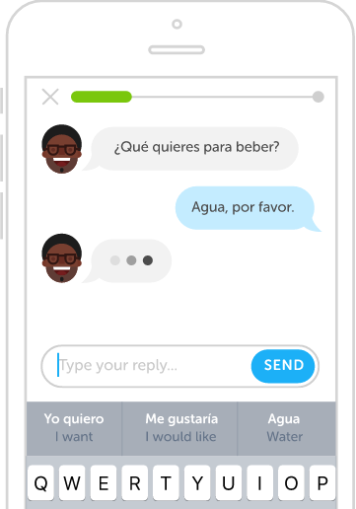
\includegraphics[width=0.3\textwidth]{duolingo}
\caption{Conversa\c tie cu chatbot folosind Duolingo}
\end{figure}

\subsection{Facebook Messenger}

\paragraph{}
Facebook s-a al\u aturat \^ intru totul afacerii conversa\c tionale, astfel \^ inc\^ at \c si-a transformat aplica\c tia Messenger \^ intr-un business de mesagerie \cite{facebook-messenger}. Compania a integrat pla\c tile peer-to-peer \^ in Messenger \^ in anul 2015, apoi urm\^ and s\u a lanseze un API pentru chatbots, astfel \^ inc\^ at business-urile s\u a poat\u a crea interac\c tiuni pentru clien\c ti. Po\c ti comanda flori, s\u a navighezi printre ultimele trend-uri \^ in materie de mod\u a, s\u a comanzi Uber, toate din\u auntrul chat-ului de Messenger (Figura 2.2).

\begin{figure}[H]
\centering
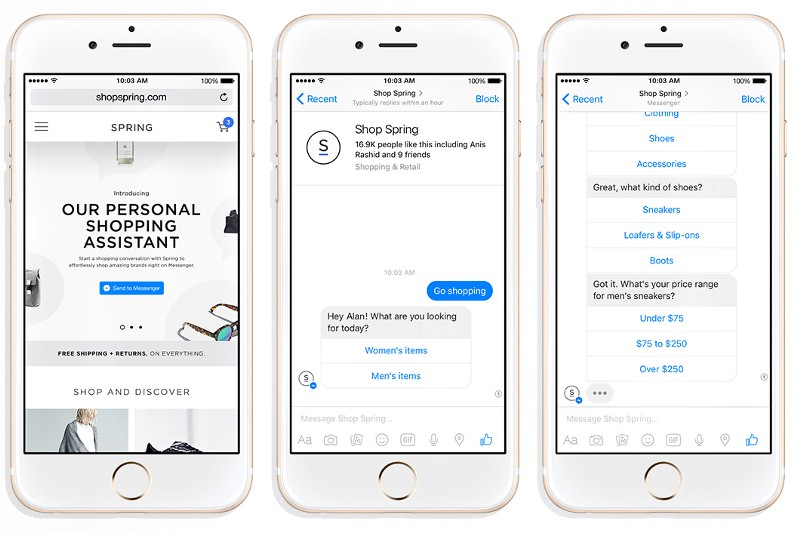
\includegraphics[width=0.7\textwidth]{facebook}
\caption{Cumpar\u aturi de haine folosind chatbot-ul companiei Spring pe Facebook Messenger}
\end{figure}


\section{Modele generative}

\paragraph{}
Spre deosebire de modelele anterioare, cele generative nu se bazeaz\u a pe r\u aspunsuri predefinite ci genereaz\u a noi r\u aspunsuri pornind de la zero. Modelele generative folosesc deobicei tehnici din Machine Translation, dar \^ in loc de a traduce dintr-o limb\u a \^ intr-alta, vom "traduce" de la o intrare la o ie\c sire (r\u aspuns). Acestea ofer\u a o mai bun\u a impresie de comunicare cu un om real. Totu\c si, ele sunt extrem de greu de antrenat, sunt predispuse la erori gramaticale (\^ in special unde lungimea propozi\c tiei este mai mare) \c si necesit\u a o cantitate mare de date de antrenare \cite{wildml-chatbots}.

\paragraph{}
Prezentul este \^ inc\u a sub semnul \^ intreb\u arii pentru acest tip de model, \^ ins\u a \^ in urm\u atorii ani, acestea vor c\u ap\u ata tot mai mult\u a aten\c tie \c si popularitate devenind tot mai performante. Dac\u a un chatbot va dobor\^ i testul Turing, \c sansele ca acesta s\u a fie generativ sunt destul de mari. Deoarece modelele generative reprezint\u a o arie de cercetare \^ inc\u a nefinisat\u a, acestea nu sunt folosite momentan \^ in produc\c tie. \^ In capitolul 3 vor fi prezentate diferite arhitecturi de re\c tele neurale, capabile s\u a modeleze conversa\c tii.